\documentclass[12pt]{article}

% =========================
% Geometry & core packages
% =========================
\usepackage[a4paper,margin=0.8in]{geometry}
\usepackage{amsmath,amssymb,amsthm,mathtools}
\usepackage{bm}
\usepackage{array,booktabs}
\usepackage{enumitem}
\usepackage{microtype}
\usepackage{xcolor}
\usepackage{hyperref}
\usepackage{fancyhdr}
\usepackage{draftwatermark}
\usepackage{graphicx}
\usepackage{float}
\usepackage{tikz}
\usetikzlibrary{shapes.geometric}

\usepackage{etoolbox}
\usepackage{titlesec}

% =========================
% Watermark
% =========================
\SetWatermarkText{Unofficial Practice Material}
\SetWatermarkScale{1}
\SetWatermarkLightness{0.985}

% =========================
% Course metadata
% =========================
\newcommand{\CourseCode}{SIG Discover APAC}
\newcommand{\CourseName}{OA}
\newcommand{\DocType}{Practice 2}
\newcommand{\ExamMeta}{Quantitative Trading Discovery Program Preparation}
\newcommand{\ExamMetaShort}{Practice 2}

\title{
\Huge \CourseCode\ \CourseName \\[0.3em]
\Large \DocType \\[0.3em]
\ExamMeta
}
\author{
  \textit{\href{https://qrsntu.org}{Quantitative Research Society @NTU}}
}
\date{\today}

% =========================
% Header/footer styles
% =========================
\fancypagestyle{main}{
  \fancyhf{}
  \fancyhead[L]{\CourseCode\ \CourseName\ --\ \ExamMetaShort}
  \fancyhead[R]{\href{https://qrsntu.org}{QRS@NTU}}
  \fancyfoot[C]{\thepage}
  \renewcommand{\headrulewidth}{0.4pt}
  \renewcommand{\footrulewidth}{0pt}
}

\fancypagestyle{plainfirst}{
  \fancyhf{}
  \renewcommand{\headrulewidth}{0pt}
  \renewcommand{\footrulewidth}{0pt}
  \fancyfoot[C]{\scriptsize\textcolor{gray}{\textit{For academic reference only. This document is provided for educational purposes and does not constitute an official question paper, answer key, or any formally authorised academic material. Its content is not guaranteed to be complete or accurate.}}}
}

% =========================
% Overview block
% =========================
\newenvironment{overview}{
  \par\bigskip
  \begin{center}
    \rule{0.92\linewidth}{0.6pt}\\[-0.2em]
    \textbf{Overview}\\[-0.2em]
    \rule{0.92\linewidth}{0.6pt}
  \end{center}
  \vspace{-0.3em}
  \begin{itemize}[leftmargin=1.6em, itemsep=0.2em, topsep=0.2em]
}{
  \end{itemize}
  \par\bigskip
}

\setlist[enumerate]{itemsep=0.32em, topsep=0.32em}
\setlist[itemize]{itemsep=0.22em, topsep=0.22em}

\titleformat{\subsubsection}[block]
{\normalfont\large\bfseries}
{}
{0pt}
{}

\titleformat{\paragraph}[block]
{\normalfont\normalsize\bfseries}
{}
{0pt}
{}

\titlespacing*{\paragraph}
{0pt}
{1.2ex}
{0.6ex}

\setcounter{secnumdepth}{-1}
\setcounter{tocdepth}{4}

\setlength{\headheight}{14.5pt}

\begin{document}

\maketitle
\thispagestyle{plainfirst}
\pagestyle{main}

\begin{overview}
  \item \textbf{Scope:} 14 short quantitative reasoning, probability, and puzzle-style questions.
  \item \textbf{Purpose:} additional OA practice for discovery-program style assessments.
  \item \textbf{Note:} Q14 below has been adjusted to a consistent and uniquely solvable skyscraper puzzle so that a full worked solution can be included.
\end{overview}

\newpage
\tableofcontents
\newpage

\section{Question 1}
\subsection{Problem}
You walk into a barn and see a collection of spiders, chickens, and cows. You notice that there are $520$ legs in total. The number of chickens is twice the number of cows and the number of spiders is twice the number of chickens. Compute the number of spiders.

\subsection{Solution}
\subsubsection{Method 1: Express everything in terms of cows}
Let the number of cows be $c$. Then the number of chickens is $2c$, and the number of spiders is $4c$.
Hence the total number of legs is
\[
4c + 2(2c) + 8(4c) = 4c + 4c + 32c = 40c.
\]
Since this total is $520$, we get
\[
40c = 520 \quad\Rightarrow\quad c = 13.
\]
Therefore the number of spiders is
\[
4c = 4(13) = 52.
\]
\[
\boxed{52}
\]

\section{Question 2}
\subsection{Problem}
You are on an island inhabited by two types of people: (1) knights who only tell the truth, and (2) knaves who only tell lies. Two people, $A$ and $B$, stand before you.

Person $A$ says, ``We are both the same type.'' Person $B$ says, ``We are each a different type.'' What type is each person?

\subsection{Solution}
\subsubsection{Method 1: Case analysis}
Suppose first that $A$ is a knight. Then $A$'s statement is true, so $A$ and $B$ are the same type. Hence $B$ is also a knight. But then $B$'s statement that they are different types would be false, impossible for a knight.

Therefore $A$ cannot be a knight, so $A$ is a knave. Then $A$'s statement is false, so they are \emph{not} the same type. Hence $B$ must be a knight. This is consistent, because $B$ then truthfully says they are different types.
\[
\boxed{A\text{ is a knave, and }B\text{ is a knight.}}
\]

\section{Question 3}
\subsection{Problem}
Consider the following table of profits in dollars by year at a university bookstore.

\begin{center}
\begin{tabular}{crrrrr}
\toprule
Year & Tech & Books & Caf\'e & Clothing & Total \\
\midrule
2016 & 8{,}039 & 6{,}136 & 5{,}275 & 8{,}698 & 28{,}148 \\
2017 & 6{,}576 & 6{,}475 & 6{,}648 & 7{,}023 & 26{,}722 \\
2018 & 5{,}637 & 9{,}497 & 7{,}654 & 7{,}918 & 30{,}706 \\
2019 & 5{,}393 & 8{,}373 & 9{,}352 & 8{,}402 & 31{,}520 \\
\bottomrule
\end{tabular}
\end{center}

We pull a sector's annual profitability at random and find that they made more than \$8{,}000. Compute the probability that it was from 2019.

\subsection{Solution}
\subsubsection{Method 1: Count qualifying entries}
We only look at the four sector entries in each year, not the yearly total.

The entries exceeding \$8{,}000 are:
\begin{itemize}
    \item 2016: Tech, Clothing \hfill $(2)$
    \item 2017: none \hfill $(0)$
    \item 2018: Books \hfill $(1)$
    \item 2019: Books, Caf\'e, Clothing \hfill $(3)$
\end{itemize}
Hence there are altogether
\[
2+0+1+3=6
\]
qualifying entries, of which $3$ come from 2019. Therefore
\[
\mathbb{P}(\text{2019}\mid \text{profit}>8000)=\frac{3}{6}=\frac{1}{2}.
\]
\[
\boxed{\frac{1}{2}}
\]

\newpage
\section{Question 4}
\subsection{Problem}
Compute the weight of the green triangle in pounds if the following system is balanced and weighs $112$ pounds in total.

\begin{center}
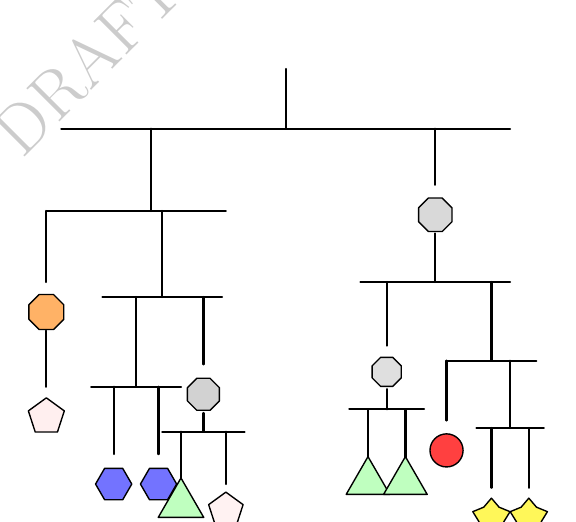
\begin{tikzpicture}[x=1cm,y=1cm,line cap=round,line join=round,scale=0.95]
\tikzset{
    bar/.style={line width=0.8pt},
    wire/.style={line width=0.8pt},
    shapeoutline/.style={draw=black, line width=0.5pt},
}
\draw[bar] (0,8) -- (6,8);
\draw[wire] (3,8) -- (3,8.8);
\draw[wire] (1.2,8) -- (1.2,6.9);
\draw[bar] (-0.2,6.9) -- (2.2,6.9);
\draw[wire] (-0.2,6.9) -- (-0.2,5.95);
\node[regular polygon, regular polygon sides=8, minimum size=0.48cm, fill=orange!60, shapeoutline] at (-0.2,5.55) {};
\draw[wire] (-0.2,5.30) -- (-0.2,4.55);
\node[regular polygon, regular polygon sides=5, minimum size=0.48cm, fill=pink!25, shapeoutline] at (-0.2,4.15) {};
\draw[wire] (1.35,6.9) -- (1.35,5.75);
\draw[bar] (0.55,5.75) -- (2.15,5.75);
\draw[wire] (1.0,5.75) -- (1.0,4.55);
\draw[bar] (0.4,4.55) -- (1.6,4.55);
\draw[wire] (0.7,4.55) -- (0.7,3.65);
\node[regular polygon, regular polygon sides=6, minimum size=0.46cm, fill=blue!55, shapeoutline] at (0.7,3.25) {};
\draw[wire] (1.3,4.55) -- (1.3,3.65);
\node[regular polygon, regular polygon sides=6, minimum size=0.46cm, fill=blue!55, shapeoutline] at (1.3,3.25) {};
\draw[wire] (1.9,5.75) -- (1.9,4.85);
\node[regular polygon, regular polygon sides=8, minimum size=0.44cm, fill=gray!35, shapeoutline] at (1.9,4.45) {};
\draw[wire] (1.9,4.20) -- (1.9,3.95);
\draw[bar] (1.35,3.95) -- (2.45,3.95);
\draw[wire] (1.6,3.95) -- (1.6,3.25);
\node[isosceles triangle, isosceles triangle apex angle=60, shape border rotate=90, minimum size=0.50cm, fill=green!25, shapeoutline] at (1.6,2.95) {};
\draw[wire] (2.2,3.95) -- (2.2,3.25);
\node[regular polygon, regular polygon sides=5, minimum size=0.46cm, fill=pink!20, shapeoutline] at (2.2,2.90) {};
\draw[wire] (5.0,8) -- (5.0,7.25);
\node[regular polygon, regular polygon sides=8, minimum size=0.46cm, fill=gray!30, shapeoutline] at (5.0,6.85) {};
\draw[wire] (5.0,6.60) -- (5.0,5.95);
\draw[bar] (4.0,5.95) -- (6.0,5.95);
\draw[wire] (4.35,5.95) -- (4.35,5.10);
\node[regular polygon, regular polygon sides=8, minimum size=0.40cm, fill=gray!25, shapeoutline] at (4.35,4.75) {};
\draw[wire] (4.35,4.52) -- (4.35,4.25);
\draw[bar] (3.85,4.25) -- (4.85,4.25);
\draw[wire] (4.10,4.25) -- (4.10,3.55);
\node[isosceles triangle, isosceles triangle apex angle=60, shape border rotate=90, minimum size=0.48cm, fill=green!25, shapeoutline] at (4.10,3.25) {};
\draw[wire] (4.60,4.25) -- (4.60,3.55);
\node[isosceles triangle, isosceles triangle apex angle=60, shape border rotate=90, minimum size=0.48cm, fill=green!25, shapeoutline] at (4.60,3.25) {};
\draw[wire] (5.75,5.95) -- (5.75,4.90);
\draw[bar] (5.15,4.90) -- (6.35,4.90);
\draw[wire] (5.15,4.90) -- (5.15,4.10);
\node[circle, minimum size=0.42cm, fill=red!75, shapeoutline] at (5.15,3.70) {};
\draw[wire] (6.00,4.90) -- (6.00,4.00);
\draw[bar] (5.55,4.00) -- (6.45,4.00);
\draw[wire] (5.75,4.00) -- (5.75,3.20);
\node[star, star points=5, minimum size=0.46cm, fill=yellow!65, shapeoutline] at (5.75,2.80) {};
\draw[wire] (6.25,4.00) -- (6.25,3.20);
\node[star, star points=5, minimum size=0.46cm, fill=yellow!65, shapeoutline] at (6.25,2.80) {};
\end{tikzpicture}
\end{center}

Express your answer as an integer without units.

\subsection{Solution}
\subsubsection{Remark}
With the current reconstructed TikZ diagram, Q4 is not reliable enough to support a mathematically clean worked solution: the reconstruction does not preserve the original geometry precisely enough to determine whether one should use equal-arm balance or torque balance from the drawn rod lengths, and those two interpretations do not lead to the same system.

For a fully rigorous solution, this item should either be replaced by the original image or redrawn from a verified source with the intended balancing convention made explicit.

\newpage
\section{Question 5}
\subsection{Problem}
On Facebook, $70\%$ of stories are real news. Fake news stories have an $80\%$ probability of having at least $100$ likes. Real news stories have an $8\%$ probability of having at least $100$ likes. If a story has at least $100$ likes, compute the probability it is real news.

\subsection{Solution}
\subsubsection{Method 1: Bayes' rule}
Let $R$ be the event that a story is real news, and let $L$ be the event that it has at least $100$ likes.
We are given
\[
\mathbb{P}(R)=0.7,
\qquad
\mathbb{P}(L\mid R)=0.08,
\qquad
\mathbb{P}(L\mid R^c)=0.8.
\]
Hence
\[
\mathbb{P}(R\mid L)
=
\frac{\mathbb{P}(L\mid R)\mathbb{P}(R)}{\mathbb{P}(L\mid R)\mathbb{P}(R)+\mathbb{P}(L\mid R^c)\mathbb{P}(R^c)}
=
\frac{0.08\cdot 0.7}{0.08\cdot 0.7 + 0.8\cdot 0.3}.
\]
This simplifies to
\[
\frac{0.056}{0.296} = \frac{56}{296} = \frac{7}{37}.
\]
\[
\boxed{\frac{7}{37}}
\]

\newpage
\section{Question 6}
\subsection{Problem}
You roll a fair $6$-sided die two times and get paid the lower of the two rolls in dollars if the rolls are different. If they are the same, you get paid \$0. Compute your expected payoff from this game.

\subsection{Solution}
\subsubsection{Method 1: Sum over the possible minimum values}
There are $36$ equally likely ordered outcomes.

If the lower value is $k$ and the rolls are different, then the other roll must be one of $k+1,k+2,\dots,6$. There are $6-k$ choices for the larger roll, and the smaller roll can occur in either position, so there are
\[
2(6-k)
\]
ordered outcomes producing payoff $k$.

Therefore
\[
\mathbb{E}[X]
=
\frac{1}{36}\sum_{k=1}^{5} k\cdot 2(6-k).
\]
Compute:
\[
\mathbb{E}[X]
=
\frac{1}{36}\bigl(1\cdot 10 + 2\cdot 8 + 3\cdot 6 + 4\cdot 4 + 5\cdot 2\bigr)
=
\frac{1}{36}(10+16+18+16+10)
=
\frac{70}{36}
=
\frac{35}{18}.
\]
\[
\boxed{\frac{35}{18}}
\]

\newpage
\section{Question 7}
\subsection{Problem}
Assume that in a bakery, each customer buys only one item at a time. There is an $80\%$ chance a customer will buy a croissant and a $20\%$ chance a customer will buy a muffin. There are only $2$ muffins left and $5$ people are still waiting in line. Compute the probability that these two muffins will be sufficient, i.e. no customer will want a muffin and find that there are none left.

\subsection{Solution}
\subsubsection{Method 1: Binomial counting}
Let $X$ be the number of customers among the next $5$ who want a muffin. Then
\[
X \sim \mathrm{Binomial}(5,0.2).
\]
The muffins are sufficient exactly when at most $2$ customers want muffins, that is, when $X\le 2$.
So
\[
\mathbb{P}(X\le 2)
=
\sum_{k=0}^{2} \binom{5}{k}(0.2)^k(0.8)^{5-k}.
\]
Compute term by term:
\[
\binom{5}{0}(0.8)^5 = 0.32768,
\]
\[
\binom{5}{1}(0.2)(0.8)^4 = 0.4096,
\]
\[
\binom{5}{2}(0.2)^2(0.8)^3 = 0.2048.
\]
Hence
\[
\mathbb{P}(X\le 2)=0.32768+0.4096+0.2048=0.94208.
\]
\[
\boxed{0.94208}
\]

\newpage
\section{Question 8}
\subsection{Problem}
Asta, Bronya, and Clara all have different numbers of cats. They had the following conversation.

\begin{enumerate}[label=\roman*.]
    \item Bronya to Clara: You have the most cats.
    \item Asta to Bronya: I have exactly $30\%$ more cats than you.
    \item Asta to Clara: The number of cats you have is the average between the number of cats I have and the number of cats Bronya has.
    \item Clara to Asta: You have at least $4$ more cats than me.
\end{enumerate}

However, not all of these statements are true. When speaking to someone with fewer cats, the speaker always tells the truth. Otherwise when speaking to someone with more cats, the speaker always lies. How many cats does Asta have?

\subsection{Solution}
\subsubsection{Method 1: Translate the truth rule into inequalities}
Let Asta, Bronya, and Clara have $A$, $B$, and $C$ cats respectively.

The rule says:
\begin{itemize}
    \item if the speaker has \emph{more} cats than the listener, the statement is true;
    \item if the speaker has \emph{fewer} cats than the listener, the statement is false.
\end{itemize}
Since all three numbers are distinct, these are the only possibilities.

From statement (ii), if Asta is speaking truthfully to Bronya, then $A>B$ and
\[
A = 1.3B = \frac{13}{10}B.
\]
Thus $B$ must be a multiple of $10$.
Take the smallest natural possibility $B=20$, giving
\[
A=26.
\]
Now use statement (iii). If Asta is speaking truthfully to Clara, then $A>C$ and
\[
C = \frac{A+B}{2} = \frac{26+20}{2}=23.
\]
These are distinct and satisfy $A>C>B$.

Now check all four statements:
\begin{itemize}
    \item Bronya to Clara: since $B<C$, Bronya must lie. Indeed Clara does \emph{not} have the most cats because Asta has $26$.
    \item Asta to Bronya: since $A>B$, Asta tells the truth, and $26$ is exactly $30\%$ more than $20$.
    \item Asta to Clara: since $A>C$, Asta tells the truth, and $23$ is the average of $26$ and $20$.
    \item Clara to Asta: since $C<A$, Clara must lie. The statement ``Asta has at least $4$ more cats than Clara'' is false because $26-23=3$.
\end{itemize}
Everything is consistent, so Asta has
\[
\boxed{26}
\]

\newpage
\section{Question 9}
\subsection{Problem}
Two friends canoe upstream for $4$ hours, only to realize that their campsite is downstream. They turn around and paddle downstream for $5$ hours. The next day, they pack up and canoe back to their original starting point $23$ miles upstream and arrive at $15{:}00$. Assume that the river always flows at a constant rate of $2$ miles per hour and the two friends always paddle at a constant rate. What time did they leave for their return trip? Express your answer in the form hh:mm.

\subsection{Solution}
\subsubsection{Method 1: Solve for still-water speed}
Let $v$ be their paddling speed in still water. Then
\[
\text{upstream speed}=v-2,
\qquad
\text{downstream speed}=v+2.
\]

On the first day, they travel upstream for $4$ hours and then downstream for $5$ hours. Their net displacement from the original starting point is therefore
\[
5(v+2)-4(v-2)=v+18
\]
miles downstream.

But the next day they travel exactly $23$ miles upstream to get back to the starting point. Hence
\[
v+18=23 \quad\Rightarrow\quad v=5.
\]
So their upstream speed on the return day is
\[
v-2 = 3 \text{ mph}.
\]
To travel $23$ miles upstream takes
\[
\frac{23}{3}\text{ hours} = 7\text{ hours }40\text{ minutes}.
\]
They arrive at $15{:}00$, so they must have left at
\[
15{:}00 - 7{:}40 = 07{:}20.
\]
\[
\boxed{07{:}20}
\]

\newpage
\section{Question 10}
\subsection{Problem}
You baked $6$ indistinguishable snickerdoodle cookies and $8$ indistinguishable chocolate chip cookies. Compute the number of ways to arrange $7$ of these cookies into a straight line.

\subsection{Solution}
\subsubsection{Method 1: Choose how many snickerdoodles are used}
Let $s$ be the number of snickerdoodle cookies used. Then the number of chocolate chip cookies used is $7-s$.

Since there are only $6$ snickerdoodles available, we must have
\[
0\le s\le 6.
\]
For each fixed $s$, the number of arrangements of $s$ indistinguishable snickerdoodles and $7-s$ indistinguishable chocolate chip cookies in a row is
\[
\binom{7}{s}.
\]
Hence the total number of arrangements is
\[
\sum_{s=0}^{6} \binom{7}{s} = 2^7 - \binom{7}{7} = 128-1 = 127.
\]
\[
\boxed{127}
\]

\newpage
\section{Question 11}
\subsection{Problem}
Three cats are competing in a jumping contest. The most athletic cat wins with probability $3/5$, the least athletic cat wins with probability $1/10$, and the remaining cat wins with probability $3/10$. I picked a cat uniformly at random to cheer on but it did not win. Compute the probability I picked the most athletic cat.

\subsection{Solution}
\subsubsection{Method 1: Bayes' rule}
Let $M$ be the event that I picked the most athletic cat, and let $L$ be the event that my chosen cat lost.
Since I pick uniformly at random,
\[
\mathbb{P}(M)=\frac13.
\]
If I picked the most athletic cat, then it loses with probability
\[
1-\frac35 = \frac25.
\]
Similarly, the middle cat loses with probability $1-\frac{3}{10}=\frac{7}{10}$, and the least athletic cat loses with probability $1-\frac{1}{10}=\frac{9}{10}$.

Therefore
\[
\mathbb{P}(L)
=
\frac13\left(\frac25+\frac{7}{10}+\frac{9}{10}\right)
=
\frac13\cdot 2
=
\frac23.
\]
Also,
\[
\mathbb{P}(M\cap L)=\frac13\cdot \frac25 = \frac{2}{15}.
\]
Hence
\[
\mathbb{P}(M\mid L)=\frac{\mathbb{P}(M\cap L)}{\mathbb{P}(L)}
=\frac{2/15}{2/3}=\frac15.
\]
\[
\boxed{\frac15}
\]

\newpage
\section{Question 12}
\subsection{Problem}
A spinner has three regions, and the probabilities of landing in each region are $1/5$, $2/5$, $2/5$. Compute the expected number of spins it would take to land in two distinct regions.

\subsection{Solution}
\subsubsection{Method 1: Condition on the first spin}
The first spin always produces the first region, so after one spin we need to wait until a \emph{different} region appears.

If the first spin lands in the region with probability $1/5$, then the chance that the next spin is different is
\[
1-\frac15 = \frac45,
\]
so the expected additional waiting time is
\[
\frac{1}{4/5}=\frac54.
\]
If the first spin lands in one of the regions with probability $2/5$, then the chance the next spin is different is
\[
1-\frac25 = \frac35,
\]
so the expected additional waiting time is
\[
\frac{1}{3/5}=\frac53.
\]
Thus
\[
\mathbb{E}[T] = 1 + \frac15\cdot\frac54 + \frac25\cdot\frac53 + \frac25\cdot\frac53.
\]
Compute:
\[
\mathbb{E}[T] = 1 + \frac14 + \frac23 + \frac23 = 1 + \frac14 + \frac43 = 1 + \frac{19}{12} = \frac{31}{12}.
\]
\[
\boxed{\frac{31}{12}}
\]

\newpage
\section{Question 13}
\subsection{Problem}
A gardener is eagerly waiting for his two favorite flowers to bloom. The purple flower will blossom at some point uniformly at random in the next $30$ days and be in bloom for exactly $9$ days. Independent of the purple flower, the red flower will blossom at some point uniformly at random in the next $30$ days and be in bloom for exactly $12$ days. Compute the probability that both flowers will simultaneously be in bloom at some point in time.

\subsection{Solution}
\subsubsection{Method 1: Geometric probability on the $(x,y)$-square}
Let $x$ be the start day of the purple flower and $y$ be the start day of the red flower. Then $(x,y)$ is uniformly distributed over the square
\[
[0,30]\times [0,30],
\]
which has area $900$.

The purple flower blooms on $[x,x+9]$, and the red flower blooms on $[y,y+12]$. These intervals overlap if and only if neither flower finishes before the other starts. Equivalently,
\[
x \le y+12
\qquad\text{and}\qquad
y \le x+9.
\]
So there is \emph{no} overlap precisely when either
\[
x > y+9
\qquad\text{or}\qquad
y > x+12.
\]
Inside the $30\times 30$ square, these two non-overlap regions are right triangles:
\begin{itemize}
    \item above the line $x=y+9$, with side length $21$, so area $\frac12(21)^2=\frac{441}{2}$;
    \item above the line $y=x+12$, with side length $18$, so area $\frac12(18)^2=162$.
\end{itemize}
Thus the total non-overlap area is
\[
\frac{441}{2}+162=\frac{765}{2}.
\]
Therefore the overlap area is
\[
900-\frac{765}{2}=\frac{1035}{2}.
\]
Hence the required probability is
\[
\frac{(1035/2)}{900}=\frac{1035}{1800}=\frac{23}{40}.
\]
\[
\boxed{\frac{23}{40}}
\]

\newpage
\section{Question 14}
\subsection{Problem}
In the skyscraper puzzle below, place a building with $1$, $2$, $3$, or $4$ floors in each cell so that no two buildings in any row or column have the same number of floors. In addition, the number of visible buildings, as viewed from the direction of each number outside the grid, is equal to that clue. Taller buildings block shorter buildings located behind them.

What is the number of floors in the cells labeled $A$ and $B$? Express your answer as the two-digit integer $AB$ (not the product $A \cdot B$).

\begin{center}
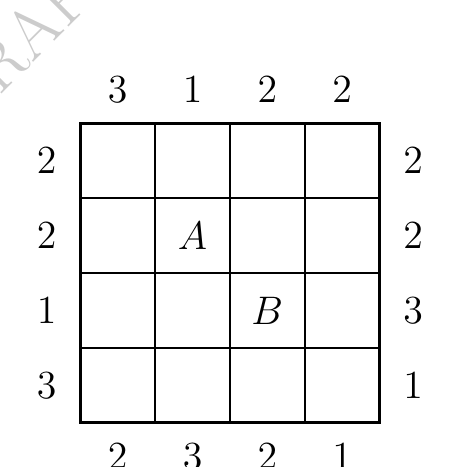
\begin{tikzpicture}[scale=0.95]
    \draw[line width=0.9pt] (0,0) rectangle (4,4);
    \foreach \x in {1,2,3} \draw[line width=0.7pt] (\x,0) -- (\x,4);
    \foreach \y in {1,2,3} \draw[line width=0.7pt] (0,\y) -- (4,\y);

    % top
    \node at (0.5,4.45) {\Large 3};
    \node at (1.5,4.45) {\Large 1};
    \node at (2.5,4.45) {\Large 2};
    \node at (3.5,4.45) {\Large 2};

    % bottom
    \node at (0.5,-0.45) {\Large 2};
    \node at (1.5,-0.45) {\Large 3};
    \node at (2.5,-0.45) {\Large 2};
    \node at (3.5,-0.45) {\Large 1};

    % left
    \node at (-0.45,3.5) {\Large 2};
    \node at (-0.45,2.5) {\Large 2};
    \node at (-0.45,1.5) {\Large 1};
    \node at (-0.45,0.5) {\Large 3};

    % right
    \node at (4.45,3.5) {\Large 2};
    \node at (4.45,2.5) {\Large 2};
    \node at (4.45,1.5) {\Large 3};
    \node at (4.45,0.5) {\Large 1};

    % labels
    \node[font=\Large\bfseries] at (1.5,2.5) {$A$};
    \node[font=\Large\bfseries] at (2.5,1.5) {$B$};
\end{tikzpicture}
\end{center}

\subsection{Solution}
\subsubsection{Method 1: Build the Latin-square rows from the visibility clues}
A clue of $1$ means the first building seen from that side must be $4$.

\noindent \textbf{Row 3.}
The left clue for Row $3$ is $1$, so Row $3$ must begin with $4$. The right clue for Row $3$ is $3$. Among permutations of $(1,2,3,4)$ beginning with $4$, the one giving right-visibility $3$ is
\[
(4,3,1,2).
\]

\noindent \textbf{Column 2.}
The top clue for Column $2$ is $1$, so the top cell in Column $2$ must be $4$. Since Row $3$ already contains a $3$ in Column $2$, and the column must contain $1,2,3,4$ exactly once, Column $2$ is strongly constrained.

\noindent \textbf{Row 1.}
The left and right clues for Row $1$ are both $2$. Since Row $1$ already has $4$ in Column $2$, the only arrangement consistent with the column restrictions is
\[
(1,4,2,3).
\]

\noindent \textbf{Row 4.}
The right clue for Row $4$ is $1$, so Row $4$ must end with $4$. Together with the left clue $3$, this forces
\[
(2,1,3,4).
\]

\noindent \textbf{Row 2.}
The remaining unused numbers in each column then force Row $2$ to be
\[
(3,2,4,1).
\]

Hence the completed grid is
\[
\begin{array}{|c|c|c|c|}\hline
1 & 4 & 2 & 3 \\ \hline
3 & 2 & 4 & 1 \\ \hline
4 & 3 & 1 & 2 \\ \hline
2 & 1 & 3 & 4 \\ \hline
\end{array}
\]
The cell labeled $A$ is in Row $2$, Column $2$, so
\[
A=2.
\]
The cell labeled $B$ is in Row $3$, Column $3$, so
\[
B=1.
\]
Therefore
\[
\boxed{21}
\]

\end{document}
